\documentclass{article}
\usepackage{graphicx, fancyhdr, amsmath}
\usepackage[margin=0.6in, top=1in]{geometry}
\usepackage{float}
\usepackage[absolute, overlay]{textpos}
\usepackage[colorlinks=true, linkcolor=blue]{hyperref}

\pagestyle{fancy}
\fancyhf{}
\renewcommand{\headrulewidth}{0pt}

\fancyhead[L]{
\begin{textblock*}{2cm}(0.3in,0.1in)  % {block width} (x-coordinate, y-coordinate)
    
\includegraphics[width=2cm]{NEW LOGO.png}  % Example image placeholder
\end{textblock*}
}
\fancyhead[R]{Math Success Program, UCLA}
\fancyfoot[R]{Created for the MSP by Asmi Kawatkar}

\fancypagestyle{plain}{
}


\title{Review Sheet: U-Substitution}
\date{}
\author{}

\begin{document}
\maketitle
\vspace{-0.75in}
\section*{Content Review}
\subsection*{Overview}

Overall procedure:
\begin{enumerate}
    \item Choose a substitution $u = g(x)$. Look for a smaller, inner expression whose derivative (or some form of the derivative) is also present in the integrand (the question given to you). Note that the goal of this substitution is to completely remove all terms in x from the integrand either through substitution or cancellation. 

    \item Compute $\frac{du}{dx} = g'(x) \Longrightarrow dx = \frac{du}{g'(x)}$

    \item Substitute in $g(x) = u$ and $dx = \frac{du}{g'(x)}$

    \item Integrate with respect to $u$

    \item If computing an indefinite integral, then replace $u$ with $g(x)$ to get the final answer. If computing a definite integral, then change the limits (demonstrated in Worked Problems)
\end{enumerate}

\subsection*{Helpful Equations}

\noindent\textit{Trigonometric/Hyperbolic Identities}
$$\sin^2\theta + \cos^2\theta = 1$$

$$\cosh^2 t - \sinh^2 t = 1$$

\noindent\textit{Integration by Parts}
$$\int{u dv} = uv - \int{v du}$$

\subsection*{Resources}


\noindent\textit{U-Subsitution}
\begin{itemize}
    \item \href{https://youtu.be/sdYdnpYn-1o}{Video: How to Integrate using U-Substitution (Organic Chemistry Tutor, 20 min) - with worked examples} 

    \item \href{https://www.khanacademy.org/math/ap-calculus-ab/ab-integration-new/ab-6-9/v/u-substitution}{U-Substitution Introduction (Khan Academy)}

    \item \href{https://youtu.be/8B31SAk1nD8}{How to Integrate using U-Substitution (NancyPi, 25 min) - with worked examples}

    \item \href{https://people.math.sc.edu/josephcf/Teaching/142/Files/Worksheets/U-Substitution.pdf}{Worksheet: University of South Carolina (with hints, challenge problems \& solutions)}

    \item \href{https://cdn.kutasoftware.com/Worksheets/Calc/05%20-%20Integration%20Substitution%20Power%20Rule.pdf}{Worksheet: U-Subsitution (with Answers)}

    \item \href{https://www.rcboe.org/cms/lib/GA01903614/Centricity/Domain/1405/u%20substitution%20WS%20solutions.pdf}{Worksheet Solutions: U-Subsitution (detailed solutions)}

    \item \href{https://www.ebnet.org/cms/lib/NJ01911729/Centricity/Domain/816/U-SUBSTITUTION-INDEFINITE-ANSWERS.pdf}{Worksheet: U-Substitution (Easy, with worked solutions)}
    
\end{itemize}


\subsection*{Acknowlegement}
Questions in the Worked Problems section of this sheet have been taken from external sources that have been linked where appropriate. Content overview  for this worksheet has been developed with reference to this \href{https://www.math.purdue.edu/~dstratma/2015.Spring.Worksheets/2015.Spring.Lecture2.Worksheet.pdf}{resource} from Purdue.  All solutions have been created independently.

\pagebreak
\section*{Worked Problems}
\label{WorkedProblems}

Compute the following indefinite integrals. 
\newline \noindent\href{https://s3.amazonaws.com/calculus-worksheets/calculus-1-tutor/Calculus+1+Tutor+-+Worksheet+11+-+Integration+by+Substitution.pdf}{Source}

\begin{enumerate}
    \item $$\int{2x\sin(x^2)} dx$$
    \begin{figure}[H]
        \centering
        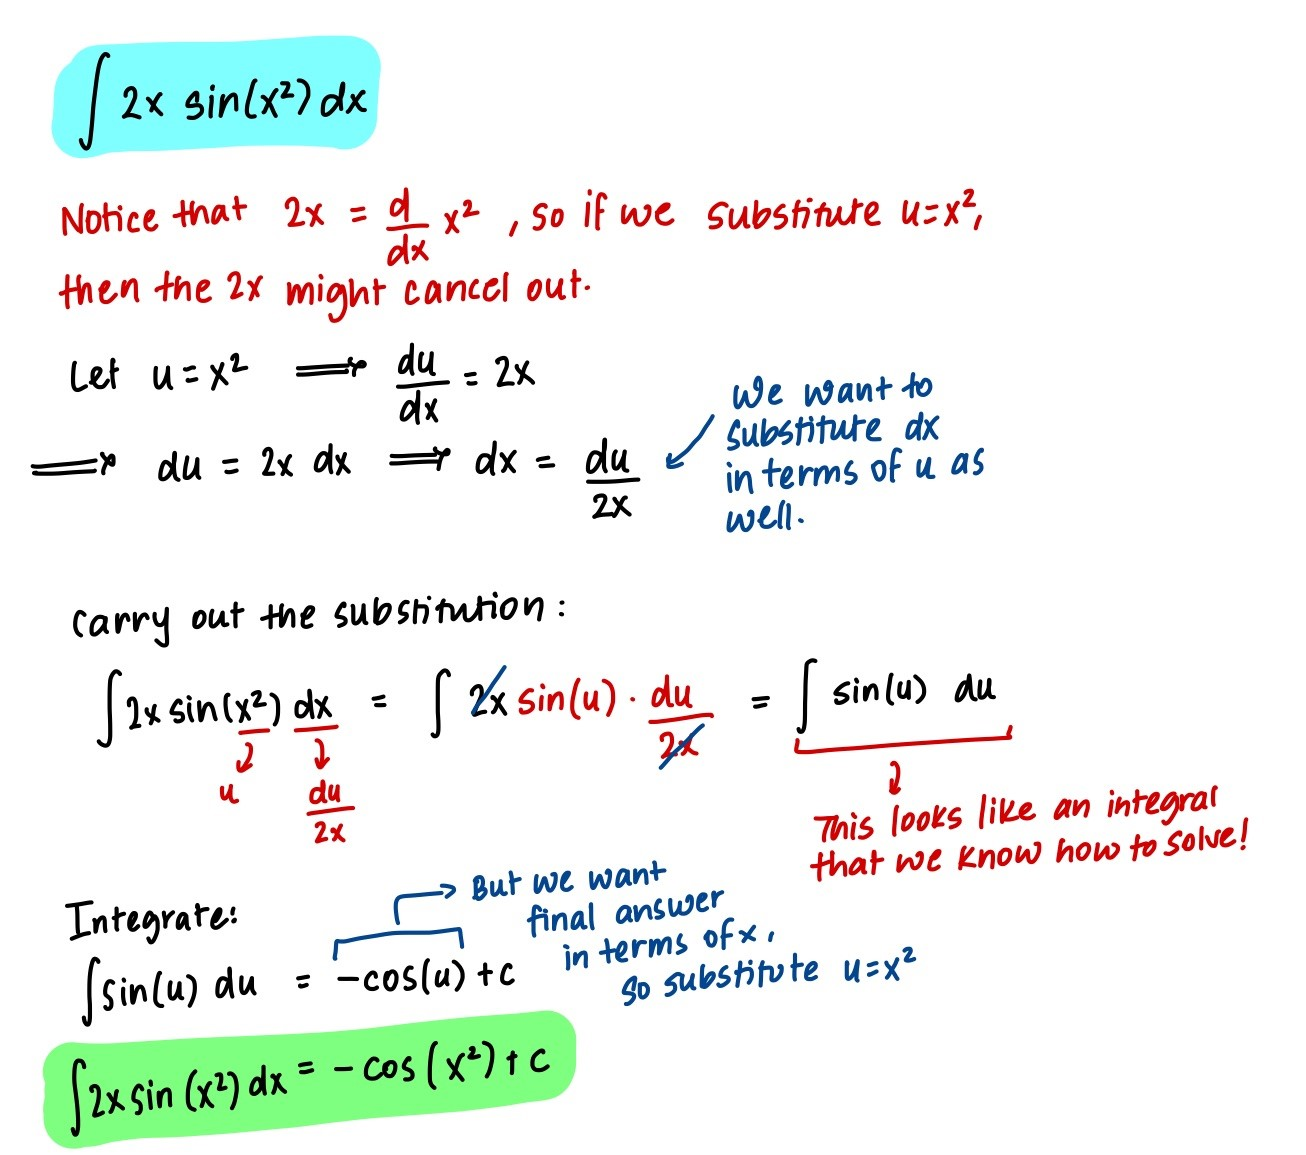
\includegraphics[width=0.6\linewidth]{Q1.jpg}
        \label{fig:Q1}
    \end{figure}
    \item $$\int{\frac{1}{x\ln x}} dx$$
    \begin{figure}[H]
        \centering
        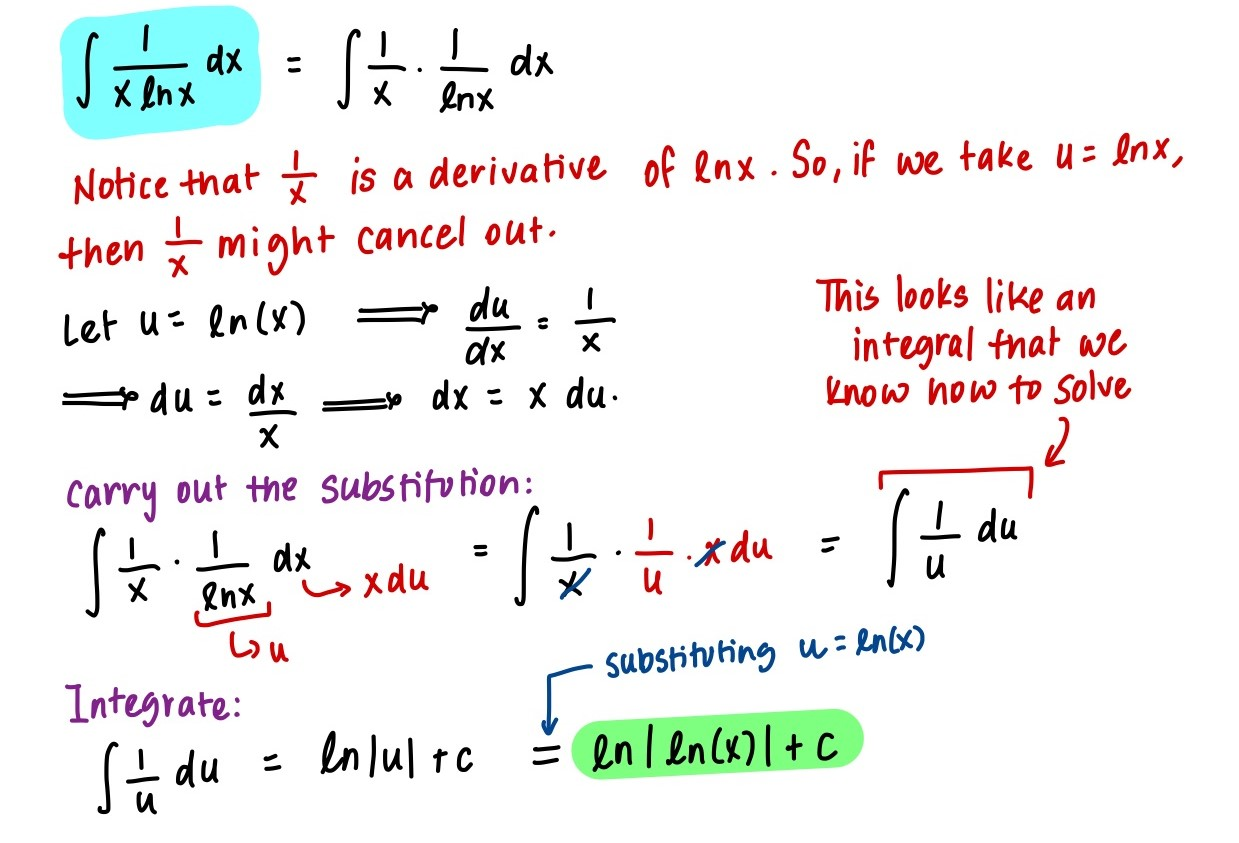
\includegraphics[width=0.6\linewidth]{Q2.jpg}
        \label{fig:Q2}
    \end{figure}
    \item $$\int{5\sqrt{5x+3}} dx$$
     \begin{figure}[H]
        \centering
        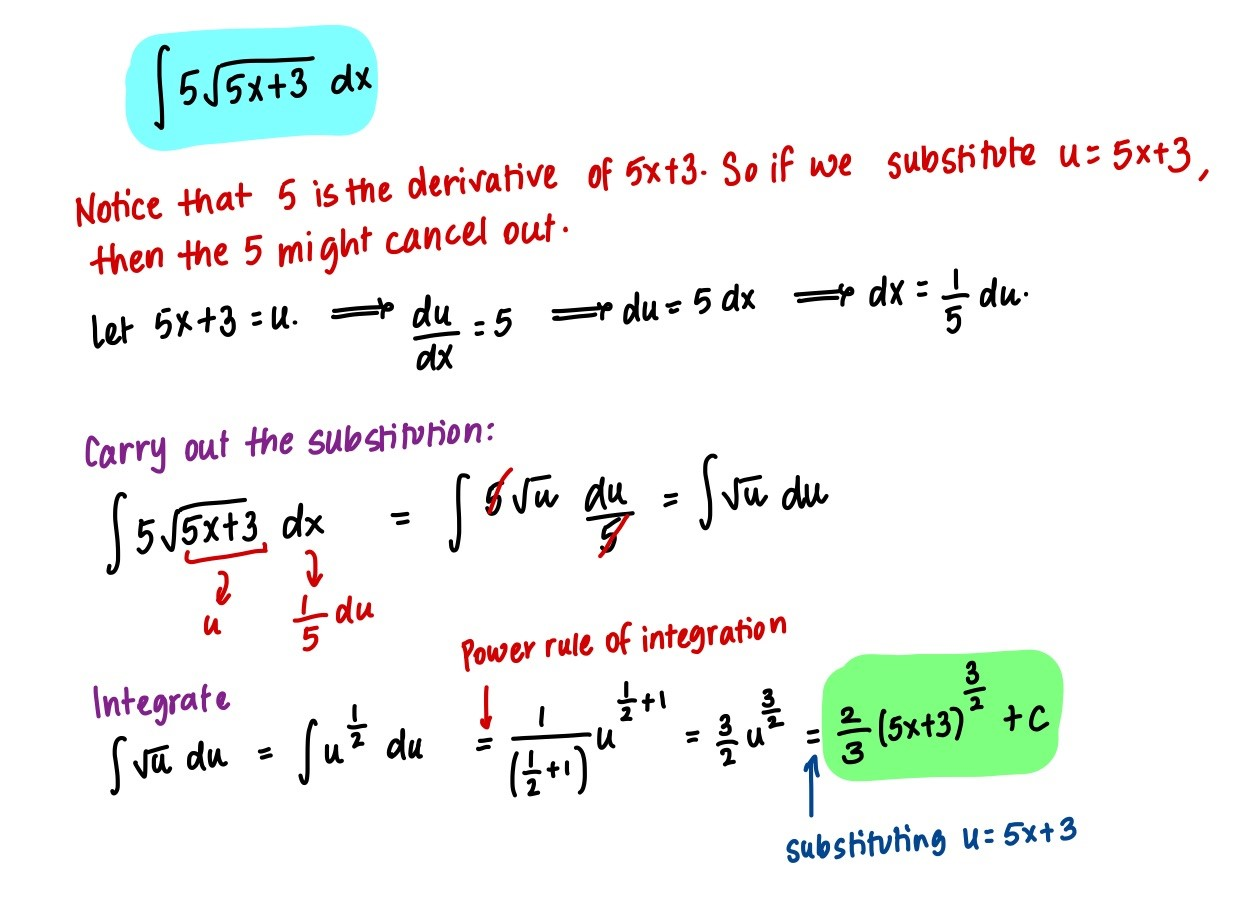
\includegraphics[width=0.8\linewidth]{Q3.jpg}
        \label{fig:Q3}
    \end{figure}
    \item $$\int{14(7x+2)^2}dx$$
     \begin{figure}[H]
        \centering
        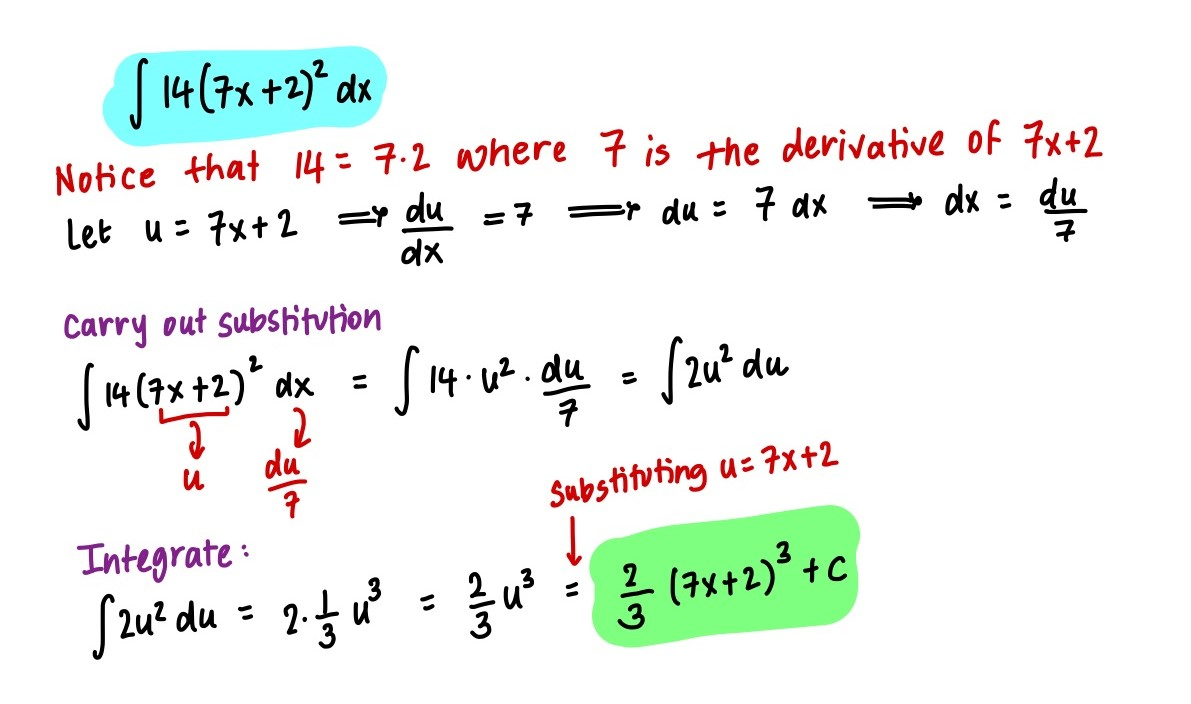
\includegraphics[width=0.8\linewidth]{Q4.jpg}
        \label{fig:Q4}
    \end{figure}
    \item $$\int{\sin^5x\cos x}dx$$
     \begin{figure}[H]
        \centering
        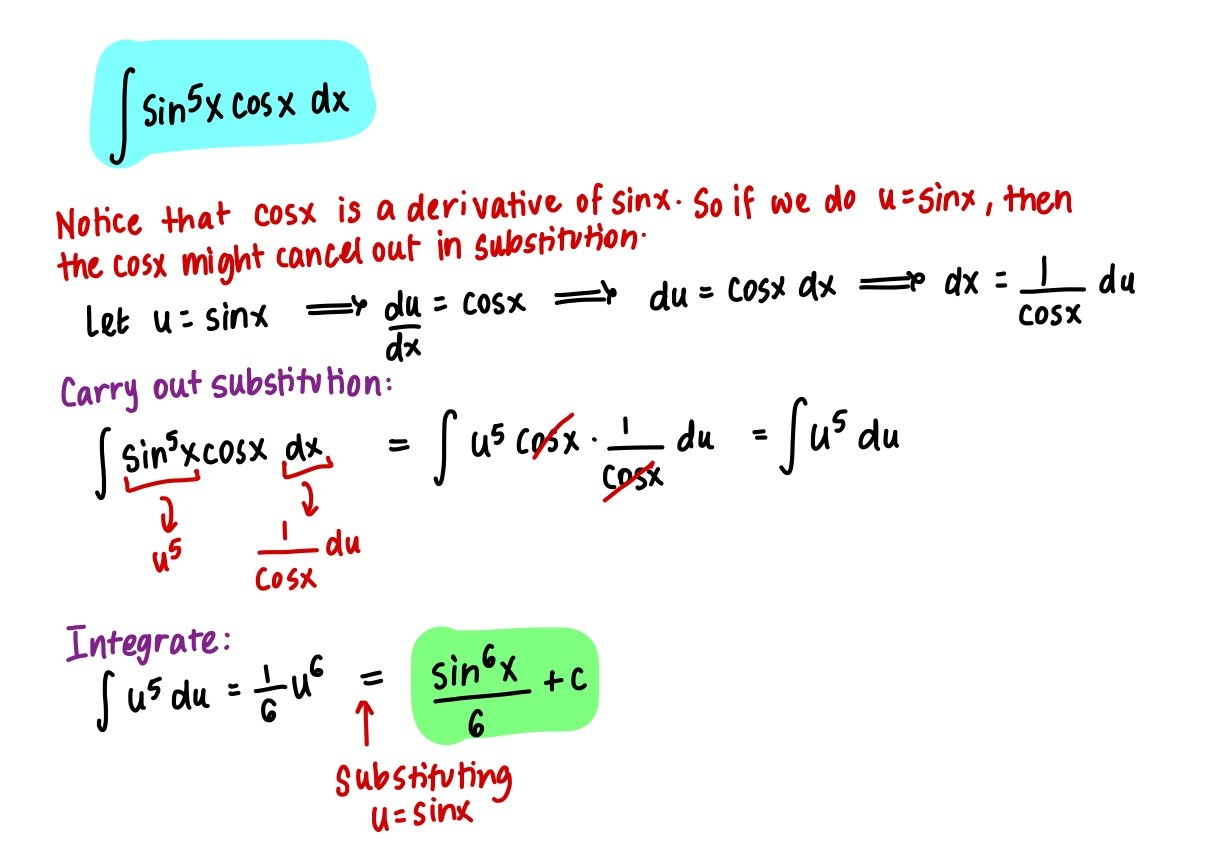
\includegraphics[width=0.7\linewidth]{Q5.jpg}
        \label{fig:Q5}
    \end{figure}
    \item $$\int{\frac{45x^2}{(3x^3+2)^4}}dx$$
     \begin{figure}[H]
        \centering
        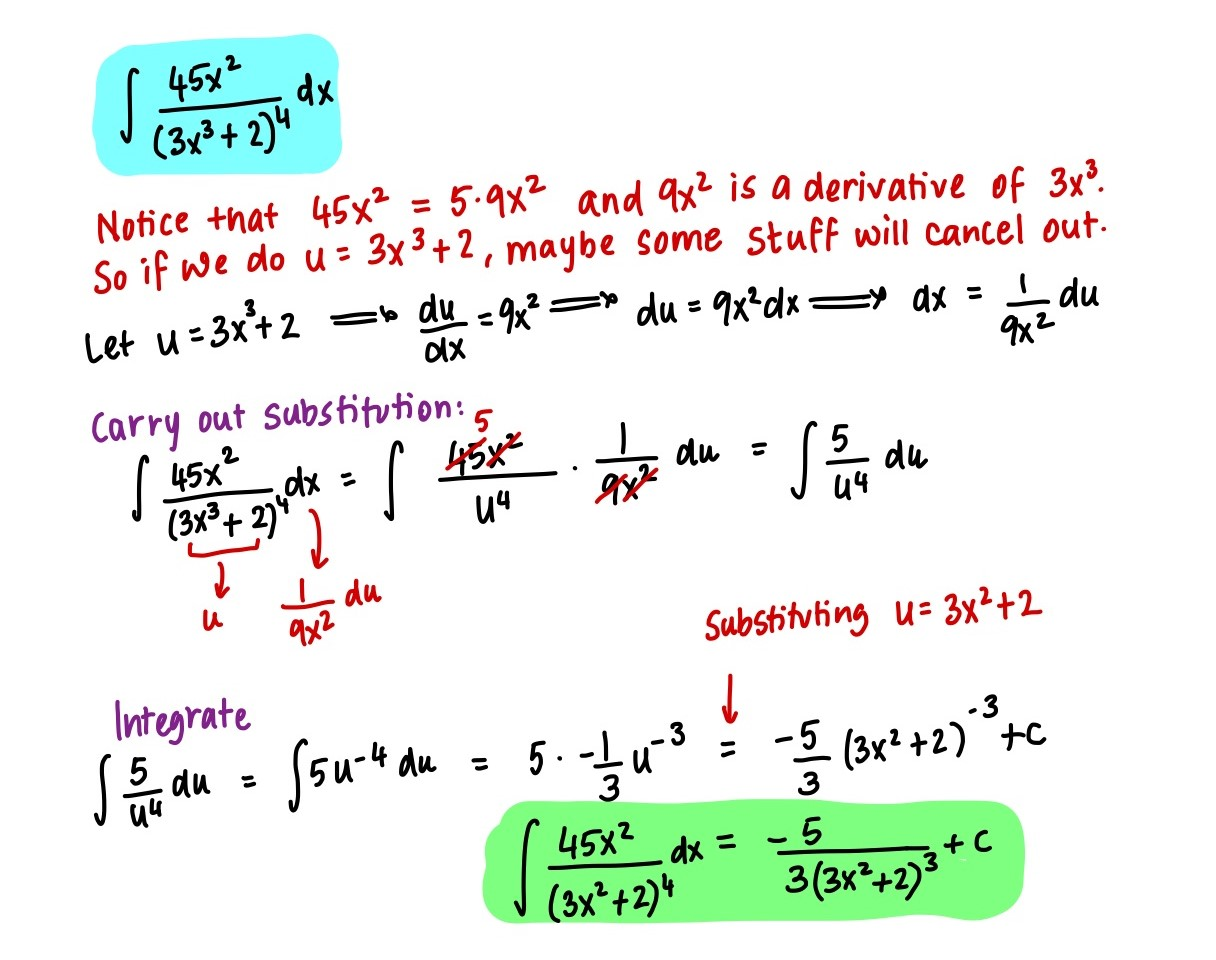
\includegraphics[width=0.7\linewidth]{Q6.jpg}
        \label{fig:Q6}
    \end{figure}
\end{enumerate}

\noindent Compute the following definite integrals.
\newline \noindent \href{https://www.math.purdue.edu/~dstratma/2015.Spring.Worksheets/2015.Spring.Lecture2.Worksheet.pdf}{Source} and another \href{https://people.math.sc.edu/josephcf/Teaching/122/Files/Handouts%20and%20Worksheets/Substitution%20+%20Definite%20Integrals.pdf}{Source}

\begin{enumerate}
    \item $$\int_0^2{\frac{x}{(x^2+25)^3}}dx$$
    \begin{figure}[H]
        \centering
        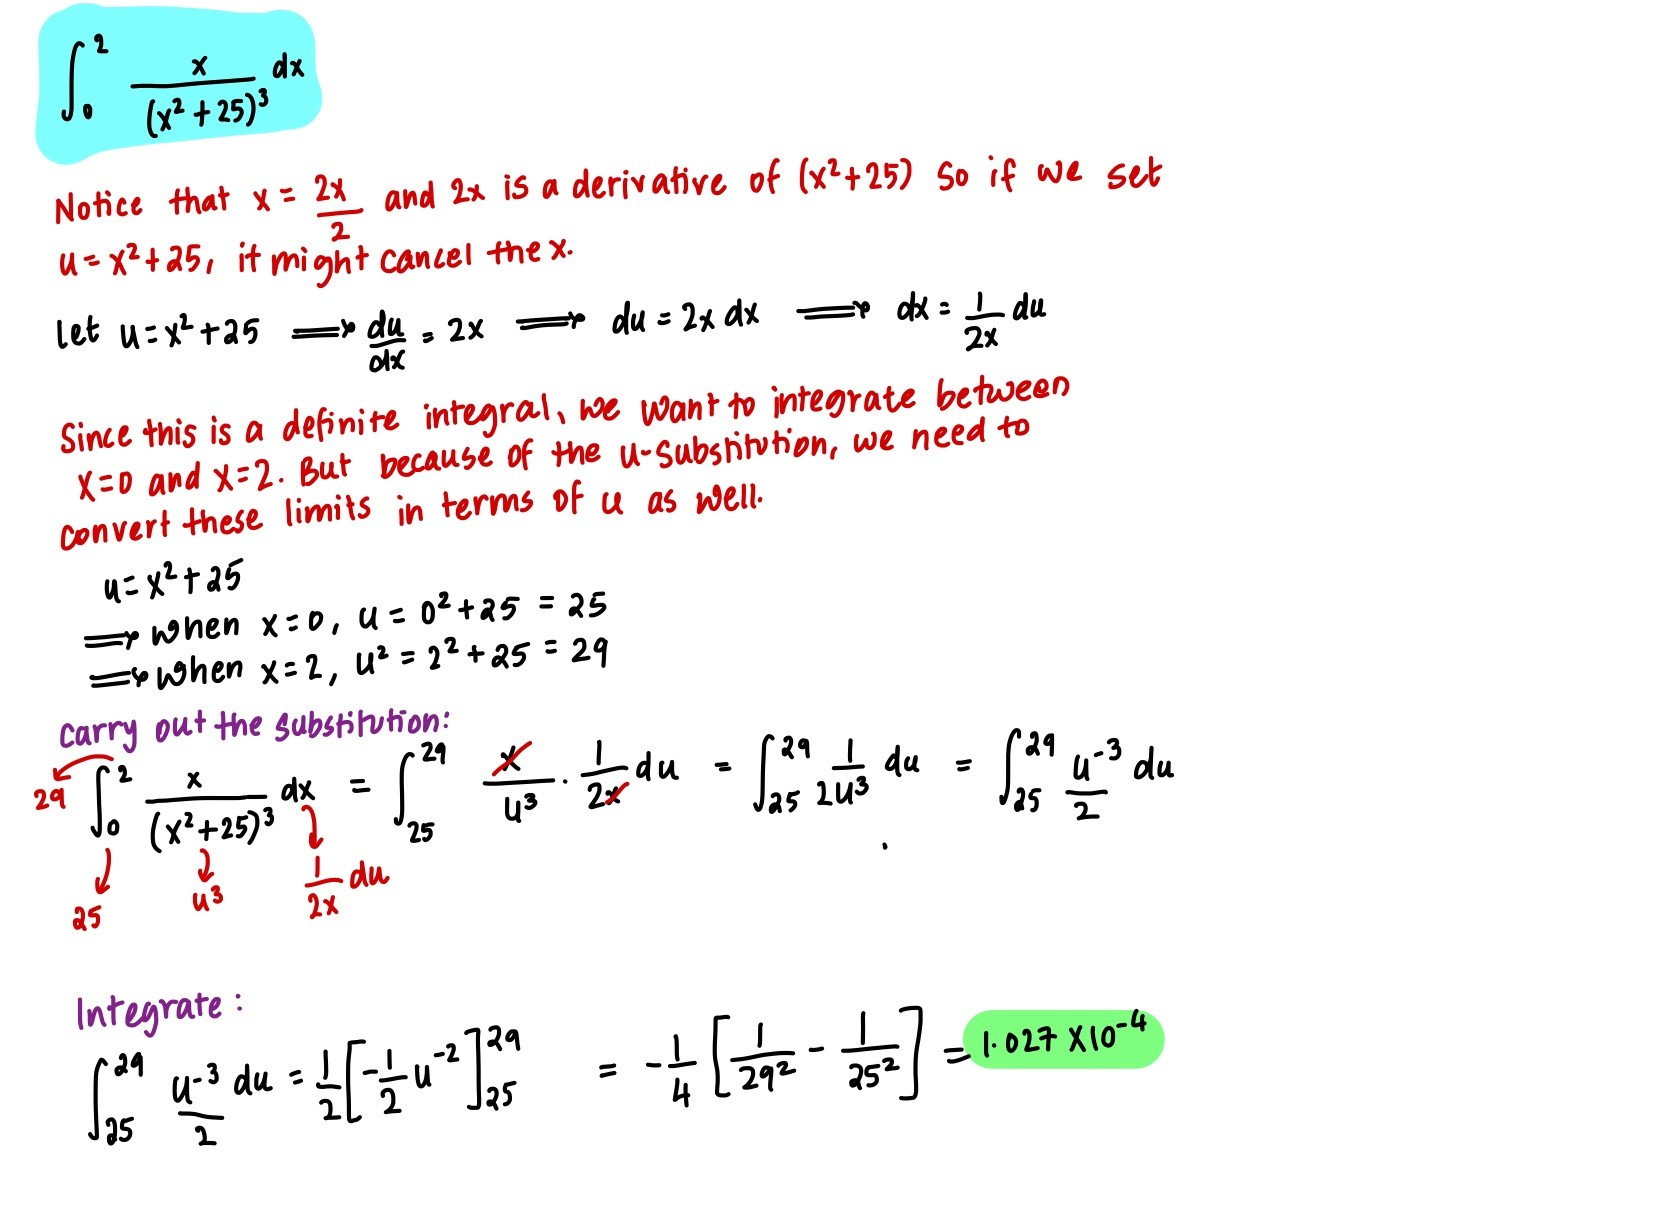
\includegraphics[width=0.7\linewidth]{Q1.1.jpg}
        \label{fig:Q1.1}
    \end{figure}
    \item $$\int_0^1{\frac{5x}{(4+x^2)^2}}dx$$
    \begin{figure}[H]
        \centering
        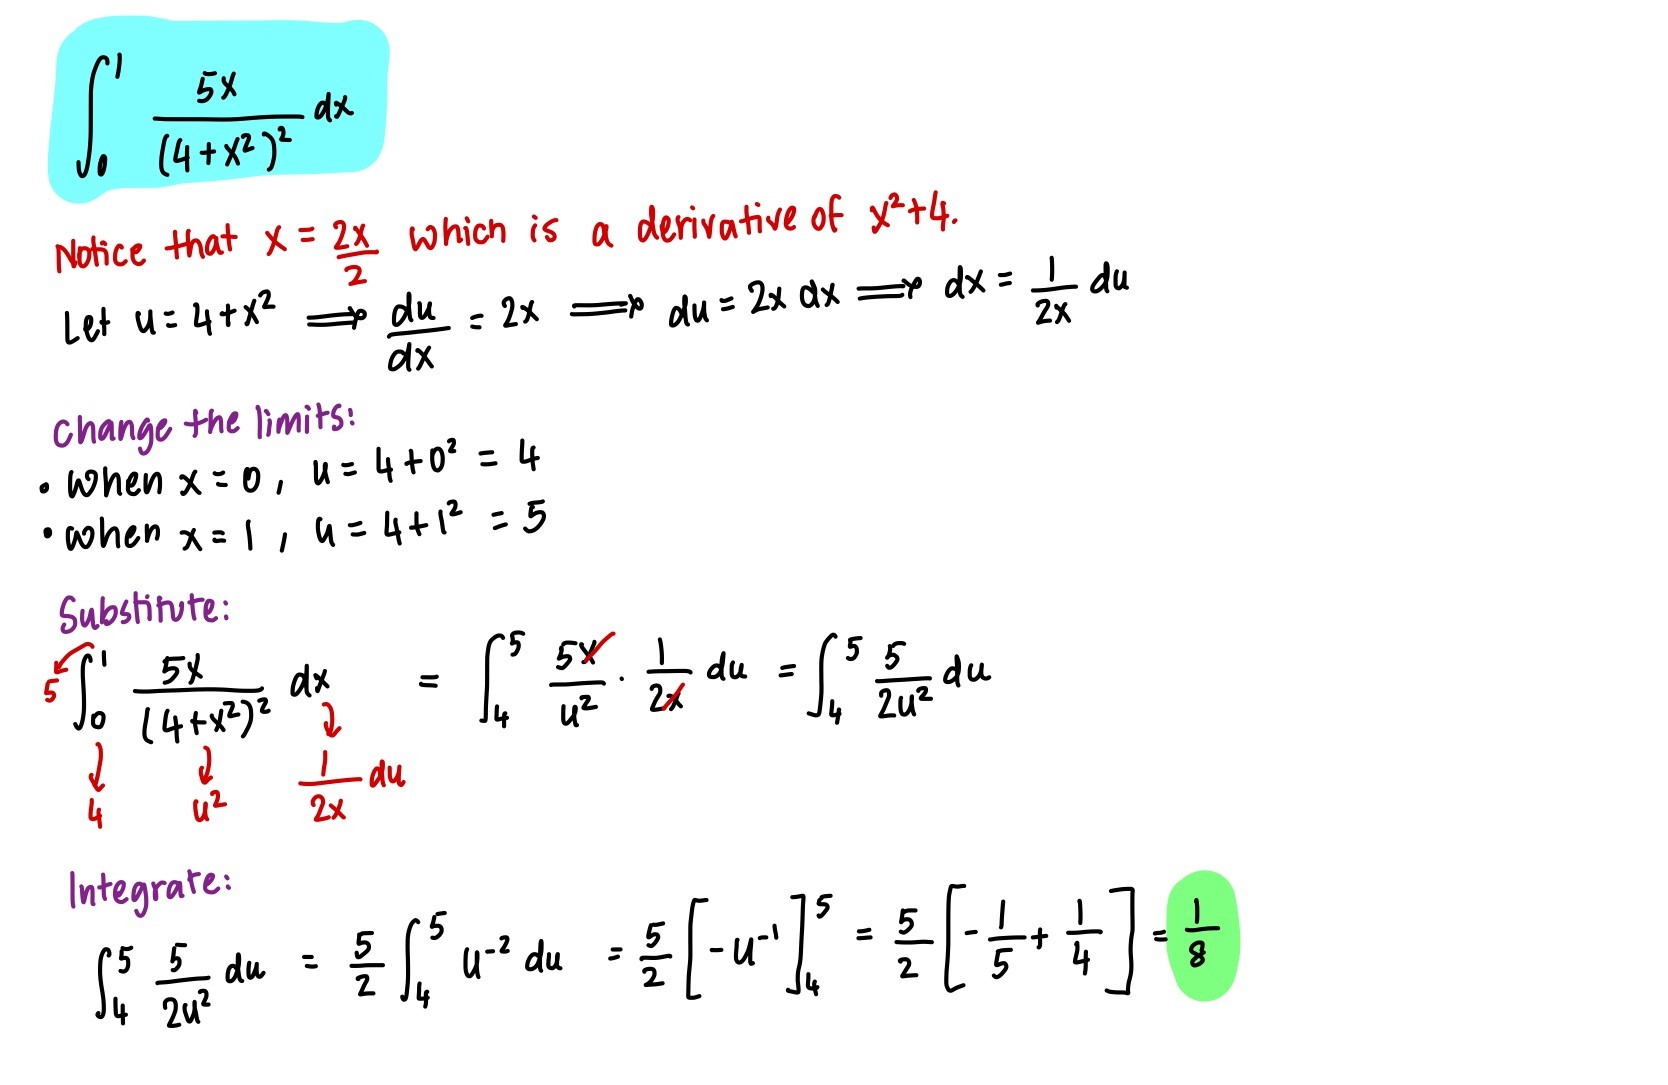
\includegraphics[width=0.7\linewidth]{Q1.2.jpg}
        \label{fig:Q1.2}
    \end{figure}
    \item $$\int_0^\pi{3\cos^3x\sin x}dx$$
    \begin{figure}[H]
        \centering
        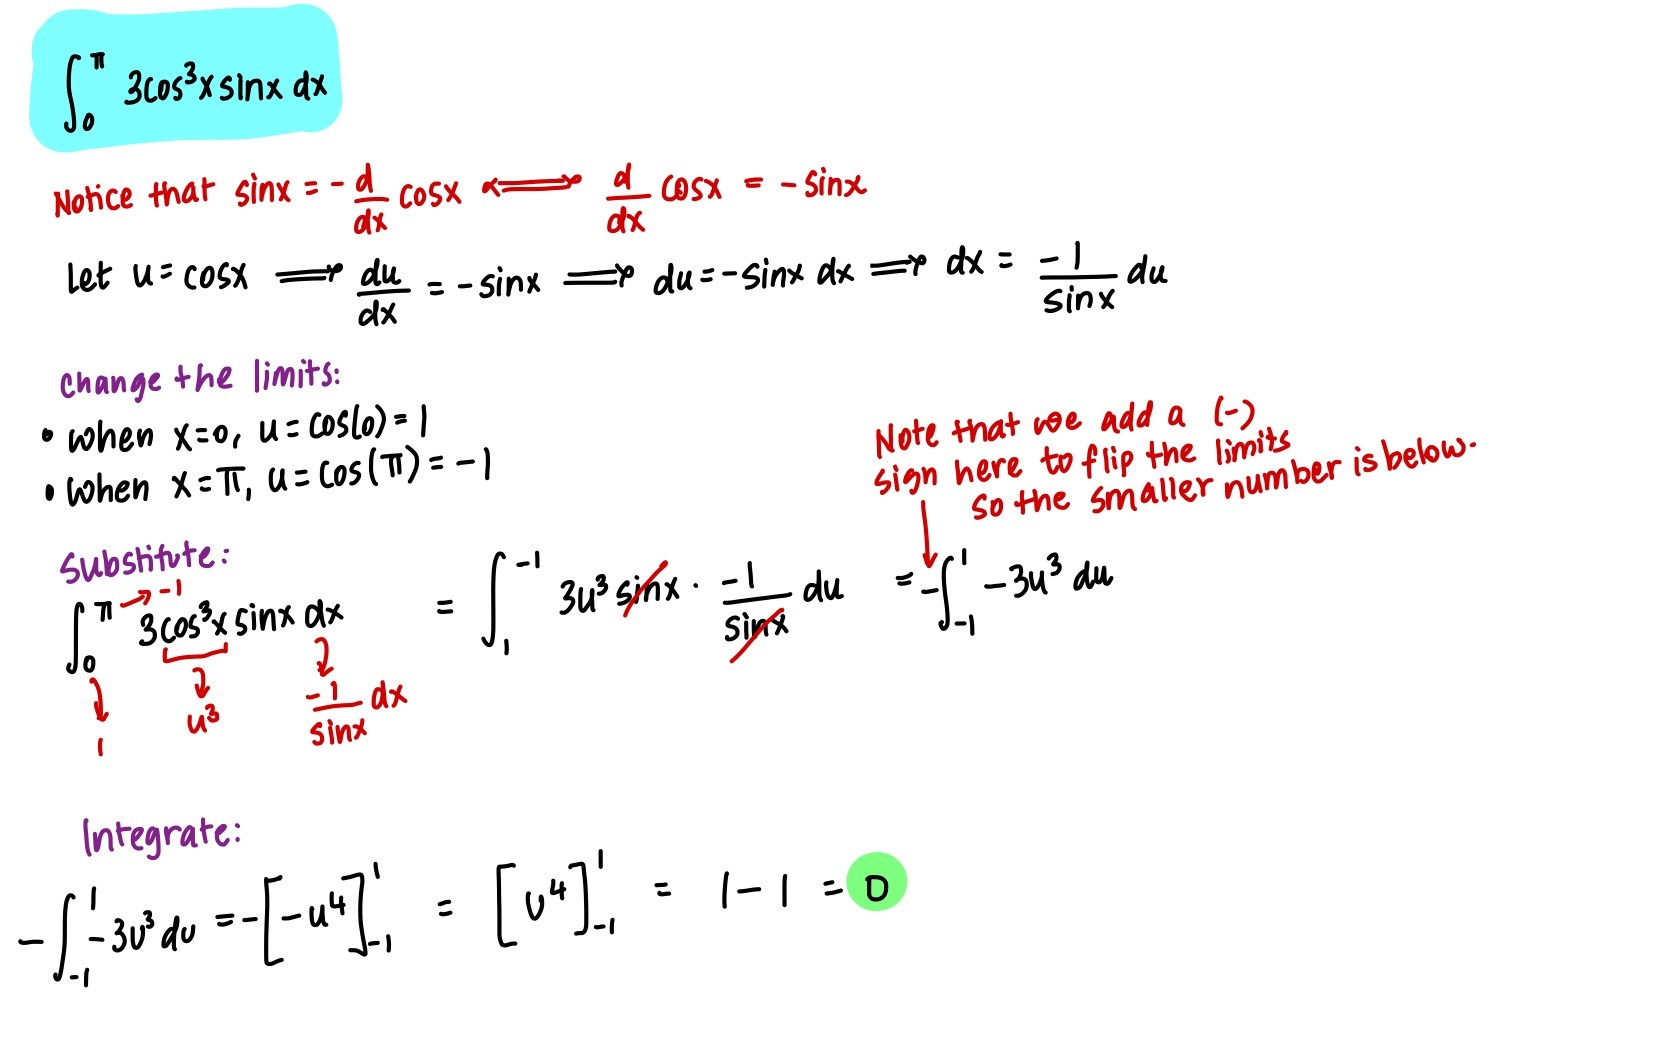
\includegraphics[width=0.7\linewidth]{Q1.3.jpg}
        \label{fig:Q1.3}
    \end{figure} 
    \item $$\int_0^1{\frac{e^{3x}}{4-e^{3x}}}dx$$
    \begin{figure}[H]
        \centering
        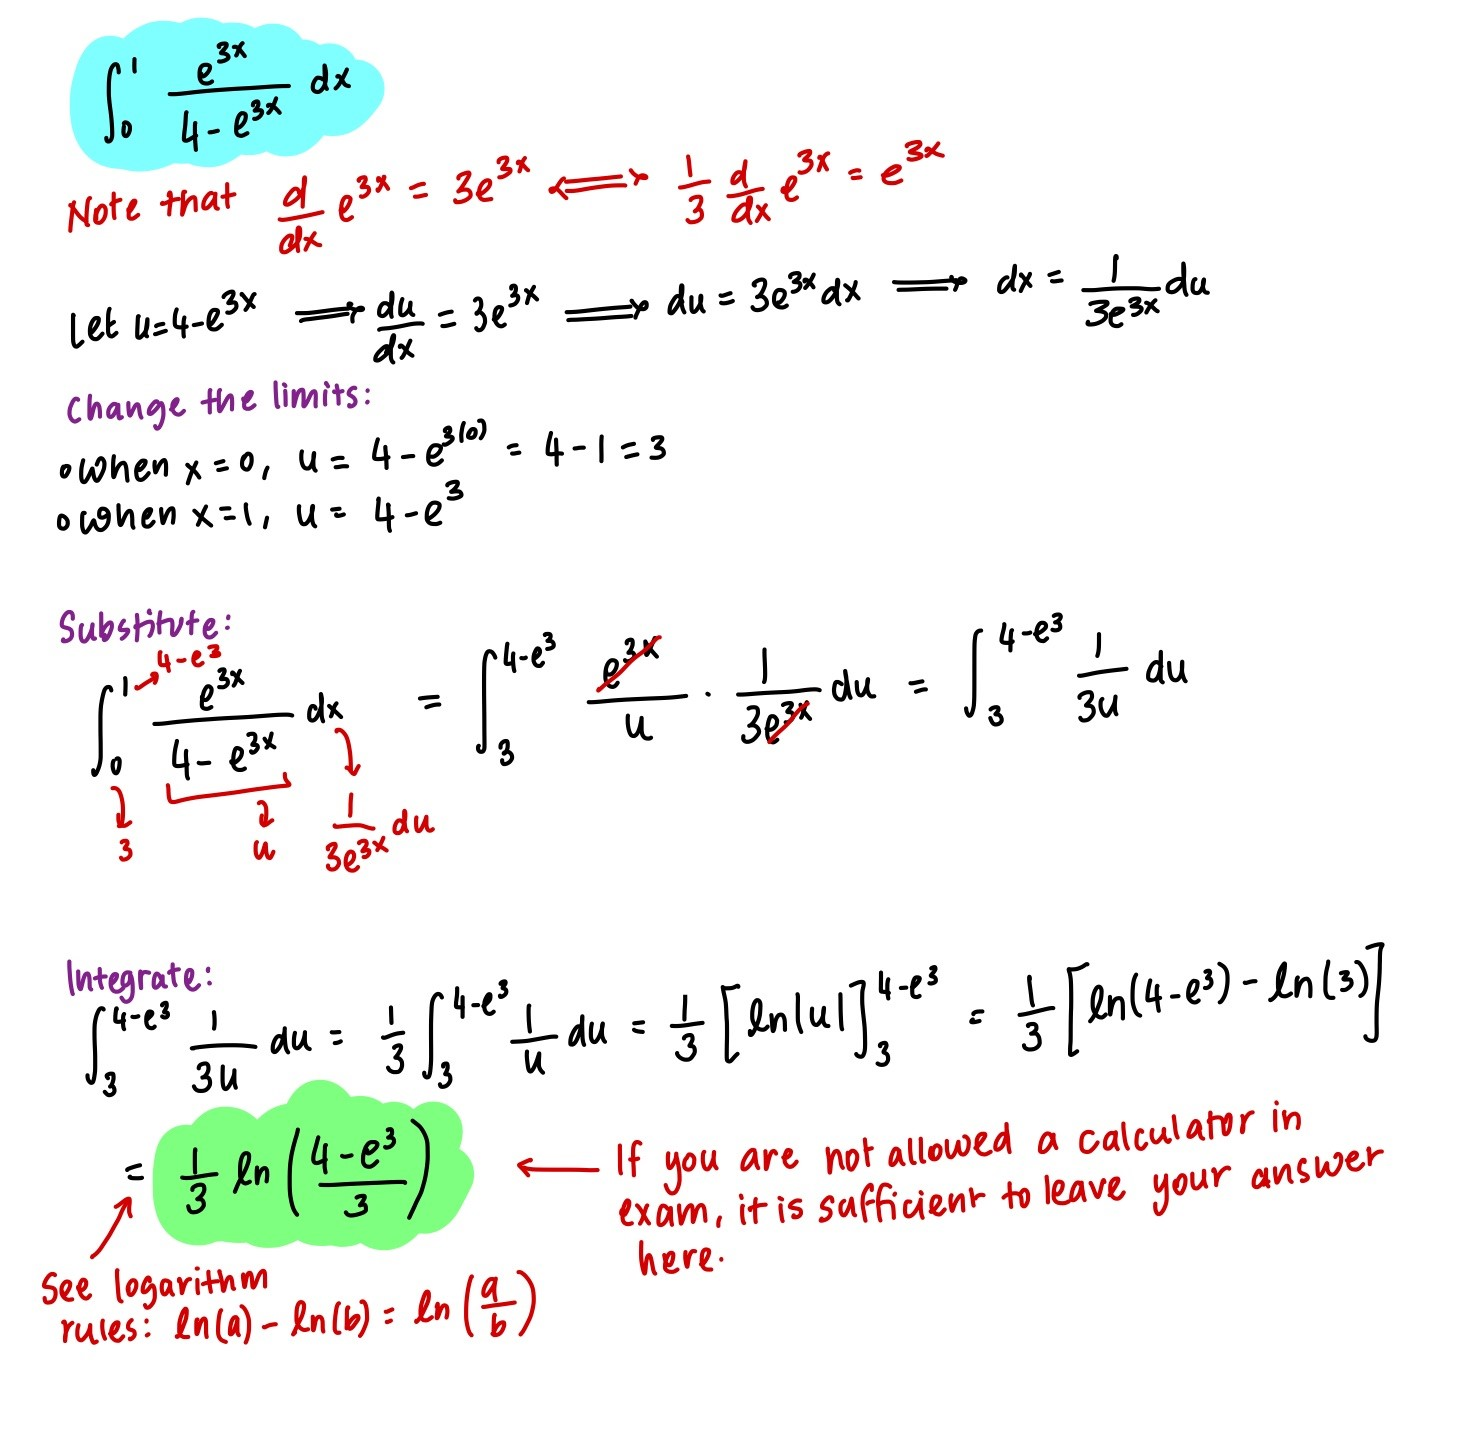
\includegraphics[width=0.6\linewidth]{Q1.4.jpg}
        \label{fig:Q1.4}
    \end{figure} 
\end{enumerate}


\end{document}
